
\documentclass[10pt]{article}
\usepackage[utf8]{inputenc}
\usepackage{kotex}
\usepackage{graphicx}
\usepackage{subfigure}
\usepackage{titling}
\setlength{\droptitle}{-2cm}
\usepackage{array}
\usepackage{amssymb}
\usepackage{amsmath}
\usepackage{siunitx} 
\usepackage{enumerate} 
\usepackage{pgfplots}
\usepackage{pgfplotstable}
\usepackage{tikz,pgfplots}
\usepackage{wasysym}
\usepackage{geometry}
\usepackage{authblk}
\usepackage{kotex}
\usepackage{bibunits}
\usepackage{tabularx}
\usepackage{hyperref}
\usepackage{pythonhighlight}

\geometry{
    a4paper,
    total={170mm,257mm},
    left=20mm,
    top=20mm,
}

\title{\textbf{MLDL : HW 1}}
\author{Jeong Min Lee}

\begin{document}
\maketitle
\section*{Notation}
\begin{enumerate}
    \item $\mathbf{v} \in \mathbb{R}^n$ : $n$ dimensional vector
    \item $\mathbf{A} \in \mathfrak{M}_{m,n}(F)$ $m\times n$ matrix. Note : $\mathfrak{M}_{m,n}(F)$ is, by definition, the set of $m \times n$ matrices over some field $F$.
    \item $v^{(i)}$ : $i$th element of vector $\mathbf{v}$
    \item $A^{(i,j)}$ : $(i,j)$ element of matrix $\mathbf{A}$
    \item $\mathfrak{L}(\boldsymbol{\beta})$ : Maximum Likelihood of parameter $\boldsymbol{\beta} \in \mathbb{R}^n$
    \item $P(X = x)$ : the probability that event $X = x$  happens
    \item $\text{diag}(\mathbf{v})$ : diagonal matrix whose diagonal entries are $\mathbf{v}$
\end{enumerate}

\section*{1}
\subsection*{(a)}
Since $P(x_i=k) = \frac{\lambda^k e^{-\lambda}}{k!}$, the MLE of Poisson probability is following.
\begin{equation}
    \mathfrak{L}(\lambda) = \prod_{k=1}^n \frac{\lambda^k e^{-\lambda}}{k!}
\end{equation}
Considering its logarithms, the MLE problem can be formalized as follow.
\begin{equation}
    \text{Maximize } \ln\mathfrak{L}(\lambda) = \sum_{k=1}^n k\ln\lambda - \lambda -\ln k!
\end{equation}
To solve the problem above, derivate it by $\lambda$ and equate to zero. The validity that such point is a solution of the MLE problem can be proved by double-derivate of $\mathfrak{L}(\lambda)$.
First of all, the first derivative of $\mathfrak{L}(\lambda)$ is as follow.
\begin{equation}
    {\partial \ln \mathfrak{L} \over \partial \lambda} = \sum_i \left(x_i/\lambda - 1\right) = 0 \quad (\because x_i = k)
    \label{eqn3}
\end{equation}
Multiplying $\lambda$ and noting that $\sum_{i=1}^n 1 = n$,equation \ref{eqn3} implies $\lambda = \frac{\sum_i x_i}{n} = \bar{x}$, where $\bar{x}$ denotes the sample mean of the data.
Furthermore, differentiate the $\ln \mathfrak{L}$ once again to check whether $\ln \mathfrak{L}$ is concave or not. 
\begin{equation}
    {\partial^2 \ln \mathfrak{L} \over \partial \lambda^2} = - \sum_i \frac{x_i}{\lambda^2}
    \label{eqn4}
\end{equation}
Since $x_i \ge 0$ and $\lambda^2 > 0$, the equation \ref{eqn3} is strictly negative, which implies that $\mathfrak{L}(\lambda)$ is concave function with respect to $\lambda$.
\subsection*{(b)}
The overall process is similar to that of problem 1-(a). First of all, the maximum likelihodd can be written as follow.
\begin{equation}
    \mathfrak{L}(\lambda) = \lambda^n \exp \left\{-\lambda \sum_{i=1}^n x_i\right\}
\end{equation}
Taking lograithms on both sides to get log likelihood gives following formula.
\begin{equation}
    \ln \mathfrak{L}(\lambda) = n\ln\lambda - \lambda \sum_i x_i
\end{equation}
Differentiate both sides by $\lambda$.
\begin{equation}
    {\partial \ln \mathfrak{L}\over \partial \lambda} = n/\lambda - \sum_i x_i = 0
\end{equation}
Therefore, $\lambda = \frac{n}{\sum_i x_i} = \bar{x}^{-1}$, which is reciprocal of sample mean of data.
The second derivative of log likelihood gives that the it is concave function, which confirm that $\lambda$ is a solution of MLE.
\begin{equation}
    {\partial^2 \ln\mathfrak{L} \over \partial \lambda^2} = -\frac{n}{\lambda^2} < 0
\end{equation}

\section*{2}
Consider $\mathbf{x}_i \in \mathbb{R}^d$ and its label $y_i \in \mathbb{R}$ for $i \in \left\{1,2,\cdots, n\right\}$. Our regression model gives the following relation.
\begin{equation}
    y_i = \mathbf{x}_i^T\boldsymbol{\beta} + \epsilon_i
\end{equation}
Suppose $\epsilon_i \sim \mathcal{N}(0,\sigma_i)$. Then, 
\begin{equation}
    y_i \sim \mathcal{N}(\mathbf{x}_i^T\boldsymbol{\beta}, \sigma_i)
\end{equation}
From the relation above, the likelihood can be written as follow.
\begin{align}
    \mathfrak{L} &= \prod_{i=1}^n P(y_i|\mathbf{x}_i,\boldsymbol{\beta})\\ 
     &= \prod_{i=1}^n \frac{1}{(2\pi)^{1/2}\sigma_i}\exp\left(-\frac{1}{2\sigma_i^2}(y_i - \mathbf{x}_i^T\boldsymbol{\beta})^2\right)\\ 
     &= \frac{1}{(2\pi)^{n/2}\sigma_1\cdots \sigma_n}\exp\left(-\sum_{i=1}^{n}\frac{1}{2\sigma_i^2}(y_i - \mathbf{x}_i^T\boldsymbol{\beta})^2\right)\\
     &= (2\pi)^{-n/2}(\det{\Sigma})^{-1/2}\exp\left(-\frac{1}{2}(\mathbf{Y - X}\boldsymbol{\beta})^T \Sigma^{-1} (\mathbf{Y - X}\boldsymbol{\beta})\right)
\end{align}
where $X = \begin{pmatrix}
    \mathbf{x}_1^T \\ \vdots \\ \mathbf{x}_n^T 
\end{pmatrix} \in \mathfrak{M}_{n,d}(\mathbb{R})$, $Y = \begin{pmatrix}
    y_1 \\ \vdots \\ y_n
\end{pmatrix} \in \mathbb{R}^n$ and $\Sigma = \text{diag}(\sigma_1^2, \cdots, \sigma_n^2)$.
The log likelihood is as follow.
\begin{equation}
    \ln \mathfrak{L} = -\frac{n}{2}\ln2\pi - \frac{1}{2}\ln\det\Sigma-\frac{1}{2}(\mathbf{Y - X}\boldsymbol{\beta})^T \Sigma^{-1} (\mathbf{Y - X}\boldsymbol{\beta})
\end{equation}
Take differentiation by $\boldsymbol{\beta}$.
\begin{equation}
    {\partial \ln \mathfrak{L}\over \partial \boldsymbol{\beta}} = -\frac{1}{2}(\mathbf{Y - X}\boldsymbol{\beta})^T(\Sigma^{-1} + (\Sigma^{-1})^T) {\partial \over \partial \boldsymbol{\beta}}\left(\mathbf{Y - X}\boldsymbol{\beta}\right)
\end{equation}
Note that ${\partial \over \partial \mathbf{x}} \mathbf{x^TAx} = \mathbf{x^T(A + A^T)}$.
\begin{align*}
    {\partial \ln \mathfrak{L} \over \partial \boldsymbol{\beta}} &= -\frac{1}{2}(\mathbf{Y - X}\boldsymbol{\beta})^T(\Sigma^{-1} + (\Sigma^{-1})^T) {\partial \over \partial \boldsymbol{\beta}}\left(\mathbf{Y - X}\boldsymbol{\beta}\right) \\
    &=  \frac{1}{2}(\mathbf{Y - X}\boldsymbol{\beta})^T(\Sigma^{-1} + (\Sigma^{-1})^T)\mathbf{X} \quad (\because {\partial \over \partial \boldsymbol{\beta}}\left(\mathbf{Y - X}\boldsymbol{\beta}\right) = -\mathbf{X}) \\
    &= (\mathbf{Y - X}\boldsymbol{\beta})^T\Sigma^{-1}\mathbf{X} \quad (\because \Sigma^{-1} = (\Sigma^{-1})^T) \\
    &= \mathbf{Y^T}\Sigma^{-1} \mathbf{X} - \boldsymbol{\beta}^T\mathbf{X^T}\Sigma^{-1}\mathbf{X} \\
    &= 0\\
    \boldsymbol{\beta^T}&\mathbf{X}^T\Sigma^{-1}\mathbf{X} = \mathbf{Y}^T\Sigma^{-1} \mathbf{X}\\
    \therefore \boldsymbol{\beta} &= \left(\mathbf{X}^T \Sigma^{-1}\mathbf{X}\right)^{-1}\left(\mathbf{X}^T\Sigma^{-1}\mathbf{Y}\right)
\end{align*}
As before, the negative definite of hessian of $\ln \mathfrak{L}$,${\partial^2 \ln \mathfrak{L} \over \partial \boldsymbol{\beta}^2}$, must be confirmed.
\begin{equation}
    {\partial^2 \ln \mathfrak{L} \over \partial \boldsymbol{\beta}^2} = - \mathbf{X}^T\Sigma^{-1}\mathbf{X}
\end{equation}
Next,$\forall \mathbf{v}\in \mathbb{R}^d$, the following condition must be held.  
\begin{equation*}
    \mathbf{v}^T{\partial^2 \ln \mathfrak{L} \over \partial \boldsymbol{\beta}^2}\mathbf{v} < 0
\end{equation*}
\begin{align*}
    \mathbf{v}^T{\partial^2 \ln \mathfrak{L} \over \partial \boldsymbol{\beta}^2}\mathbf{v} &= - \mathbf{v^TX^T}\Sigma^{-1}\mathbf{Xv} \\
    &= -\mathbf{u}\Sigma^{-1}\mathbf{u}\quad \text{where } \mathbf{u = Xv}\in \mathbb{R}^n \\
    &= -u_1^2/\sigma_1^2 - \cdots - u_n^2/\sigma_n^2 <0
\end{align*}
Thus, the proof is done.
\section*{3}
In this probelm, I'll derive the log-likelihood and its derivative to justify my implementation.
Since $x_i$ follows beta distribution, the likelihood is all product of $p_\theta(x_i)$.
\begin{equation}
    \mathfrak{L} = \prod_{i = 1}^n \frac{1}{B(\alpha,\beta)} x_i^{\alpha-1}(1-x_i)^{\beta-1}
\end{equation}
Taking a logarithm on both sides, we can derive log-likelihood.
\begin{equation}
    \ln \mathfrak{L} = \sum_i -\ln B(\alpha, \beta) + (\alpha-1)x_i + (\beta-1)(1-x_i)
\end{equation}
Since maximizing the log-likelihood is equivalent to minimizing the negative of log-likelihood, we can define it as a loss function.
\begin{equation}
    l(\alpha, \beta) = -(\alpha-1)\sum_i x_i - (\beta - 1) \sum_i(1-x_i) + N\ln B
    \label{eqn20}
\end{equation}
Refering to equation \ref{eqn20} says, I implemented \textbf{compute\_loss()} to return it. 

Then, taking a derivative with respect to $\alpha, \beta$, I computed the gradient of the loss function.
\begin{align}
    {\partial l(\alpha, \beta)\over \partial \alpha} &= N (\psi(\alpha) - \psi(\alpha + \beta)) - \sum_i \ln x_i \\
    {\partial l(\alpha, \beta)\over \partial \beta} &= N (\psi(\beta) - \psi(\alpha + \beta)) - \sum_i \ln (1-x_i)
\end{align}
Since $\sum_i x  = N\bar{x}$, I use \textbf{np.mean()} function to calculate the last term of each gradient. Please note that in the implementation, I drop the factor of $N$ since I considered the average of the gradient.
Using the gradient descent algorithm(I attached it in the appedix as well as submitted the .ipynb file), I attained the following figure. 
\clearpage
\begin{figure}[!h]
    \begin{center}
        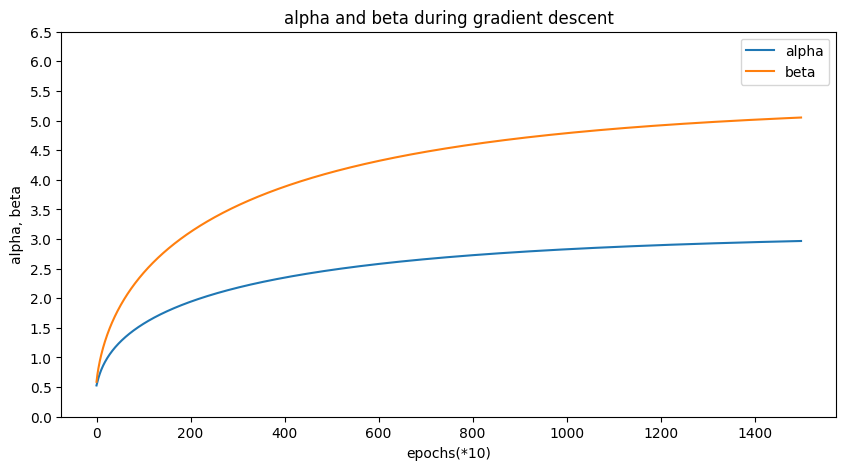
\includegraphics[scale = 0.5]{"fig/fig1.png"}
    \end{center}
    \caption{The convergence of each parameter. They are success to converge to their true values.}
    \label{fig1}
\end{figure}
As figure \ref{fig1} says, $\alpha, \beta$ converges to vicinity of their true value, 3 and 5, respectively.
Furthermore, I conducted the experiment that repeats this algorithm 100 times. From this experiment, I observed the distribution of estimate of each parameter.

\begin{figure}[!h]
    \begin{center}
        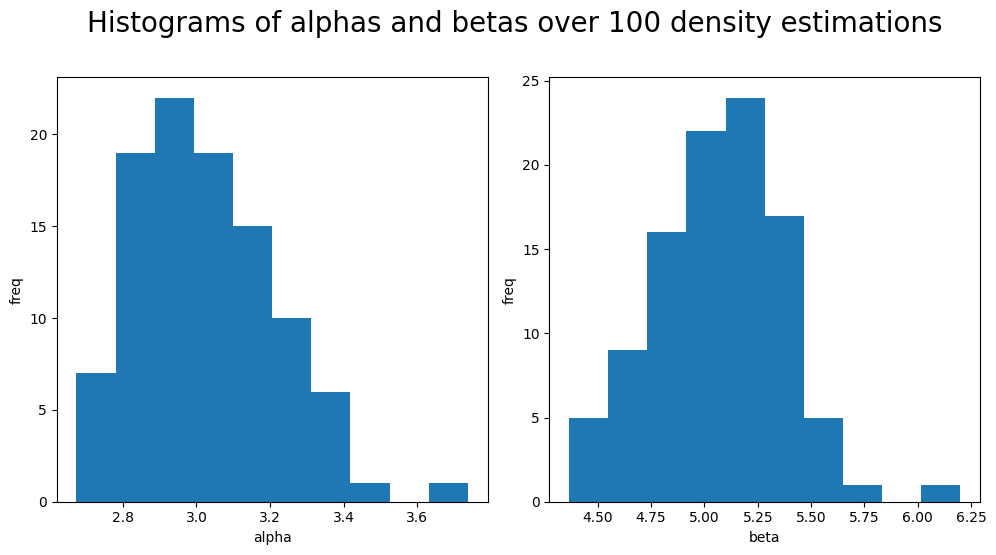
\includegraphics[scale = 0.5]{"fig/fig2.png"}
    \end{center}
    \caption{The distribution of estimated parameters}
    \label{fig2}
\end{figure}

As figure \ref{fig2} describes, the distributions of $\alpha,\beta$ are concentrated on the vicinity of their true value, respectively. 
The core statistics are listed at follows.
\begin{table}[!h]
    \begin{center}
        \begin{tabular}{lll}
            & $\alpha$ & $\beta$ \\
            \hline \hline
        mean               & 2.808                 & 4.654                \\
        standard deviation & 0.139                 & 0.205               
        \end{tabular}
        \caption{The table of the basic statistics calculated from the distribution of each parameters}
    \end{center}
\end{table}

\section*{4}
Please refer to the code I submitted or the appendix to see my implementation.
Note that I made the input $X$ as a matrix(not a sparse matrix as the skeleton code gives) to extensively deploy the matrix multiplication in my implementation.
One would be able to find that I reduce at least one summation, which corresponsds to a single for-loop, by using matrix multiplication in \textbf{fit(), predict()} function.
The test accuracy of my algorithm was about 0.98, which is pretty high. This implies that the Naive Bayes Classifier is efficient classifier that can classify the input data despite its absurd assumption.

Here, I'll discuss about problem 4-(d).
In this problem, we are looking for the probability of the word 'ossec' given that the security level is 2. The variable `model.probs` in my impelementation is a matrix that stores the estimated probabilities of each word given each class (or security level). 
We first need to find the index of the word 'ossec' in our vocabulary. Then, we can find the corresponding probability from `model.probs`,which is 1.148e-05
The reason why the estimated probability of 'ossec' given level 2 is non-zero (despite the word 'ossec' not appearing in level 2 logs) is because of the smoothing factor alpha. 
When we calculate the probabilities, we add alpha to the numerator and alpha times the number of features to the denominator. 
This prevents probabilities from being zero, which can be helpful for numerical stability and to account for possible features that did not appear in the training data but might appear in the test data. 
If alpha was set to 0, then the probability of 'ossec' given level 2 would be zero. 

\appendix
\section{Problem 3 : Implementation}
\begin{python}
class BetaDistribution:
    """ class for modeling Beta distribution over alpha, beta"""

    def __init__(self, a=0.5, b=0.5):
        """
        Initializes the model parameters: alpha and beta.

        Do NOT Modify this method.

        Inputs
        - a: alpha
        - b: beta
        """
        self.a = a
        self.b = b

    def forward(self, X):
        """
        forward pass of the model.

        Do NOT Modify this method.

        Inputs
        - X: a numpy array of training data of the shape (N,)
        Returns
        - outputs: the probability of X following the beta distribution defined by the model parameters.
        """
        beta_func = special.beta(self.a, self.b)
        outputs = 1/beta_func * np.power(X, self.a-1) * np.power(1-X, self.b-1)
        return outputs

    def compute_loss(self, X):
        """
        Computes the loss for gradient descent using the log-likelihood of the model.

        Question (a)
        - hint: use special.beta for beta function.

        Inputs
        - X: a numpy array of training data of the shape (N,)
        Returns
        - loss: a float of loss
        """
        N = X.shape[0]
        return N*(np.log(special.beta(self.a,self.b)) - (self.a-1)*np.mean(np.log(X)) - (self.b-1)*np.mean(np.log(1-X)))

    def backward(self, X):
        """
        Computes the gradients of the loss function with respect to the model parameters.

        Question (b)
        - hint: use special.polygamma for psi function.

        Inputs
        - X: a numpy array of training data of the shape (N,)
        Returns
        - gradients: a dictionary containing 'alpha' and 'beta' as keys with their corrresponding gradients as values.
        """
        N = X.shape[0]
        delta_alpha =  N*(special.polygamma(0, self.a) - special.polygamma(0,self.a + self.b) - np.mean(np.log(X)))
        delta_beta = N*(special.polygamma(0, self.b) - special.polygamma(0,self.b + self.a) - np.mean(np.log(1-X)))
        return {'alpha' : delta_alpha, 'beta' : delta_beta}

    def train(self, X, lr, n_epochs, log_interval=10):
        """
        Runs gradient descent

        Do NOT Modify this method.

        Inputs
        - X
        - lr
        - n_epochs
        - log_interval
        Returns
        - history
        """
        history = []
        for epoch in range(n_epochs):
            self.train_step(X, lr)
            if epoch % log_interval==0:
                loss = self.compute_loss(X)
                history.append((loss, self.a, self.b))
        return history

    

    def train_step(self, X, lr):
        """
        Updates the parameters using gradient descent

        Question (c)

        Inputs
        - X
        - lr: learning rate
        """
        grad = self.backward(X)
        delta_alpha = grad['alpha']
        delta_beta = grad['beta']
        self.a -= lr*delta_alpha
        self.b -= lr*delta_beta

\end{python}
\section{Problem 4 : Implementation}
\begin{python}
class MultinomialNaiveBayes:
    def __init__(self, alpha=1.0):
        """Initializes the model hyperparameter alpha(smoothing factor).
        """
        self.classes = None
        self.priors = None
        self.probs = None
        self.alpha = alpha

    def fit(self, X, y):
        """Estimates prior of classes and conditional probabilities given each class.

        Args:
            X: a numpy array of training data, shape (N, feature_dim)
            y: a numpy array of training label classes, shape (N,)
        """
        n_samples, n_features = X.shape
        self.classes = np.unique(y)
        n_classes = len(self.classes)

        self.priors = np.zeros(n_classes, dtype=np.float64)
        self.probs = np.zeros((n_classes, n_features), dtype=np.float64)

        #### Question (a) #####
        # Estimate self.priors and self.probs.
        # You must utilize self.alpha (smoothing factor)

        ##################
        # IMPLEMENT HERE #
        ##################
        for k in range(n_classes):
            self.priors[k] = self.alpha + np.sum(y == k)
        self.priors /= (n_classes * self.alpha + n_samples)

        X_sum = np.sum(X, axis=1)
        for k in range(n_classes):
            for j in range(n_features):
                self.probs[k,j] = (self.alpha + np.sum(X[y==k, j]))/ (n_features * self.alpha + np.sum(np.int64(y == k) * X_sum))

    def predict(self, X):
        """Predicts the class of input X.

        Args:
            X: a numpy array of test data, shape (N, feature_dim)

        Returns:
            y_hat: a numpy array of predicted classes, shape (N,)
        """

        #### Question (b) #####
        # Predict the class of input X using estimated self.priors and self.probs.
        # As we learned in class, it is numerically stable to use log probability instead of raw probability.

        ##################
        # IMPLEMENT HERE #
        ##################
        N,_ = X.shape
        y_hat = np.zeros(N,dtype = np.float64)
        for n in range(N):
            y_hat[n] = np.argmax(np.log(self.priors) + np.sum(np.log(self.probs)*X[n,:], axis=1))
        return y_hat
       
\end{python}
\end{document}